%% BioMed_Central_Tex_Template_v1.06
%%                                      %
%  CDAOtools.tex            ver: 1.00 %
%                                       %

%%IMPORTANT: do not delete the first line of this template
%%It must be present to enable the BMC Submission system to 
%%recognise this template!!

%%%%%%%%%%%%%%%%%%%%%%%%%%%%%%%%%%%%%%%%%
%%                                     %%
%%  LaTeX template for BioMed Central  %%
%%     journal article submissions     %%
%%                                     %%
%%         <14 August 2007>            %%
%%                                     %%
%%                                     %%
%% Uses:                               %%
%% cite.sty, url.sty, bmc_article.cls  %%
%% ifthen.sty. multicol.sty		   %%
%%				      	   %%
%%                                     %%
%%%%%%%%%%%%%%%%%%%%%%%%%%%%%%%%%%%%%%%%%


%%%%%%%%%%%%%%%%%%%%%%%%%%%%%%%%%%%%%%%%%%%%%%%%%%%%%%%%%%%%%%%%%%%%%
%%                                                                 %%	
%% For instructions on how to fill out this Tex template           %%
%% document please refer to Readme.pdf and the instructions for    %%
%% authors page on the biomed central website                      %%
%% http://www.biomedcentral.com/info/authors/                      %%
%%                                                                 %%
%% Please do not use \input{...} to include other tex files.       %%
%% Submit your LaTeX manuscript as one .tex document.              %%
%%                                                                 %%
%% All additional figures and files should be attached             %%
%% separately and not embedded in the \TeX\ document itself.       %%
%%                                                                 %%
%% BioMed Central currently use the MikTex distribution of         %%
%% TeX for Windows) of TeX and LaTeX.  This is available from      %%
%% http://www.miktex.org                                           %%
%%                                                                 %%
%%%%%%%%%%%%%%%%%%%%%%%%%%%%%%%%%%%%%%%%%%%%%%%%%%%%%%%%%%%%%%%%%%%%%


\NeedsTeXFormat{LaTeX2e}[1995/12/01]
\documentclass[10pt]{bmc_article}    



% Load packages
\usepackage{cite} % Make references as [1-4], not [1,2,3,4]
\usepackage{url}  % Formatting web addresses  
\usepackage{ifthen}  % Conditional 
\usepackage{multicol}   %Columns
\usepackage[utf8]{inputenc} %unicode support
\usepackage{graphicx}
%\usepackage[applemac]{inputenc} %applemac support if unicode package fails
%\usepackage[latin1]{inputenc} %UNIX support if unicode package fails
\urlstyle{rm}
 
 
%%%%%%%%%%%%%%%%%%%%%%%%%%%%%%%%%%%%%%%%%%%%%%%%%	
%%                                             %%
%%  If you wish to display your graphics for   %%
%%  your own use using includegraphic or       %%
%%  includegraphics, then comment out the      %%
%%  following two lines of code.               %%   
%%  NB: These line *must* be included when     %%
%%  submitting to BMC.                         %% 
%%  All figure files must be submitted as      %%
%%  separate graphics through the BMC          %%
%%  submission process, not included in the    %% 
%%  submitted article.                         %% 
%%                                             %%
%%%%%%%%%%%%%%%%%%%%%%%%%%%%%%%%%%%%%%%%%%%%%%%%%                     


%\def\includegraphic{}
%\def\includegraphics{}



\setlength{\topmargin}{0.0cm}
\setlength{\textheight}{21.5cm}
\setlength{\oddsidemargin}{0cm} 
\setlength{\textwidth}{16.5cm}
\setlength{\columnsep}{0.6cm}

\newboolean{publ}

%%%%%%%%%%%%%%%%%%%%%%%%%%%%%%%%%%%%%%%%%%%%%%%%%%
%%                                              %%
%% You may change the following style settings  %%
%% Should you wish to format your article       %%
%% in a publication style for printing out and  %%
%% sharing with colleagues, but ensure that     %%
%% before submitting to BMC that the style is   %%
%% returned to the Review style setting.        %%
%%                                              %%
%%%%%%%%%%%%%%%%%%%%%%%%%%%%%%%%%%%%%%%%%%%%%%%%%%
 

%Review style settings
\newenvironment{bmcformat}{\begin{raggedright}\baselineskip20pt\sloppy\setboolean{publ}{false}}{\end{raggedright}\baselineskip20pt\sloppy}

%Publication style settings
%\newenvironment{bmcformat}{\fussy\setboolean{publ}{true}}{\fussy}



% Begin ...
\begin{document}
\begin{bmcformat}


%%%%%%%%%%%%%%%%%%%%%%%%%%%%%%%%%%%%%%%%%%%%%%
%%                                          %%
%% Enter the title of your article here     %%
%%                                          %%
%%%%%%%%%%%%%%%%%%%%%%%%%%%%%%%%%%%%%%%%%%%%%%

%\title{CDAO Store: A New Vision for Data Integration}
\title{\emph{CDAO-Store:} Ontology-driven Data Integration for Phylogenetic Analysis}

 
%%%%%%%%%%%%%%%%%%%%%%%%%%%%%%%%%%%%%%%%%%%%%%
%%                                          %%
%% Enter the authors here                   %%
%%                                          %%
%% Ensure \and is entered between all but   %%
%% the last two authors. This will be       %%
%% replaced by a comma in the final article %%
%%                                          %%
%% Ensure there are no trailing spaces at   %% 
%% the ends of the lines                    %%     	
%%                                          %%
%%%%%%%%%%%%%%%%%%%%%%%%%%%%%%%%%%%%%%%%%%%%%%


\author{Brandon Chisham\correspondingauthor%
       \email{Brandon Chisham\correspondingauthor - bchisham@cs.nmsu.edu}%
      \and
               Ben Wright \correspondingauthor%
         \email{Ben Wright \correspondingauthor - bwright@cs.nmsu.edu}%
	\and
         Trung Le%
         \email{Trung Le - tle@cs.nmsu.edu}%
    \and
	Tran Son %
	\email{Tran Son - tson@cs.nmsu.edu}%
       and 
	Enrico Pontelli%
	\email{Enrico Pontelli -epontell@cs.nmsu.edu}%
      }
      

%%%%%%%%%%%%%%%%%%%%%%%%%%%%%%%%%%%%%%%%%%%%%%
%%                                          %%
%% Enter the authors' addresses here        %%
%%                                          %%
%%%%%%%%%%%%%%%%%%%%%%%%%%%%%%%%%%%%%%%%%%%%%%

\address{%
    Department of Computer Science, New Mexico State University, Las Cruces, New Mexico, USA
}%

\maketitle

%%%%%%%%%%%%%%%%%%%%%%%%%%%%%%%%%%%%%%%%%%%%%%
%%                                          %%
%% The Abstract begins here                 %%
%%                                          %%
%% The Section headings here are those for  %%
%% a Research article submitted to a        %%
%% BMC-Series journal.                      %%  
%%                                          %%
%% If your article is not of this type,     %%
%% then refer to the Instructions for       %%
%% authors on http://www.biomedcentral.com  %%
%% and change the section headings          %%
%% accordingly.                             %%   
%%                                          %%
%%%%%%%%%%%%%%%%%%%%%%%%%%%%%%%%%%%%%%%%%%%%%%


\begin{abstract}
        % Do not use inserted blank lines (ie \\) until main body of text.
        %This should not exceet 350 words and should be structured into separate sections headed Background, Results, Conclusions.  Please do not use abbreviations or references in the abstract.
	\paragraph*{Background:} The Comparative Data Analysis Ontology
	(CDAO) is an ontology developed, as part of the EvoInfo and
	EvoIO groups supported by NESCent,  to provide semantics
	the descriptions of data and transformations commonly found in the domain of
	phylogenetic inference. The core concepts of the ontology enables the
	description of phylogenetic trees and associated character data matrices.

        \paragraph*{Results:} Using CDAO as the semantic backend, we
        developed a triple-store, named \emph{CDAO-Store.} CDAO-Store is a RDF-based
        store of phylogenetic data, including a complete import of TreeBASE. CDAO-Store provides
        a web-based front-end to perform both user-defined as well as domain-specific
        queries; domain-specific queries include search for nearest common ancestors,
        minimum spanning clades,  filter multiple trees in the store by size, author, taxa,  
        tree identifier, algorithm or method.  In addition, CDAO-Store provides a
        visualization front-end, called \emph{CDAO-Explorer}, which can be used 
        to view both character data matrices and trees extracted from the CDAO-Store.  
        CDAO-Store provides import capabilities, enabling the addition of new data
        to the triple-store; files in PHYLIP, MEGA, and NEXUS formats can be imported and
        their CDAO representation added to the triple-store.

        \paragraph*{Conclusions:} CDAO-Store is made up of a versatile and integrated
        set of tools to support phylogenetic analysis. To the best of our knowledge, CDAO-Store
        is the first semantically-aware repository of phylogenetic data with domain-specific
        querying capabilities. The portal to CDAO-Store is available at \url{http://www.cs.nmsu.edu/~cdaostore}.
\end{abstract}



\ifthenelse{\boolean{publ}}{\begin{multicols}{2}}{}




%%%%%%%%%%%%%%%%%%%%%%%%%%%%%%%%%%%%%%%%%%%%%%
%%                                          %%
%% The Main Body begins here                %%
%%                                          %%
%% The Section headings here are those for  %%
%% a Research article submitted to a        %%
%% BMC-Series journal.                      %%  
%%                                          %%
%% If your article is not of this type,     %%
%% then refer to the instructions for       %%
%% authors on:                              %%
%% http://www.biomedcentral.com/info/authors%%
%% and change the section headings          %%
%% accordingly.                             %% 
%%                                          %%
%% See the Results and Discussion section   %%
%% for details on how to create sub-sections%%
%%                                          %%
%% use \cite{...} to cite references        %%
%%  \cite{koon} and                         %%
%%  \cite{oreg,khar,zvai,xjon,schn,pond}    %%
%%  \nocite{smith,marg,hunn,advi,koha,mouse}%%
%%                                          %%
%%%%%%%%%%%%%%%%%%%%%%%%%%%%%%%%%%%%%%%%%%%%%%




%%%%%%%%%%%%%%%%
%% Background %%
%%
\section*{Background}

The \emph{CDAO-Store} is a novel portal aimed at facilitating the storage 
and retrieval of phylogenetic data. The novelty of CDAO-Store lies in the use of a 
\emph{semantic-based}
approach to the storage and querying of data, building on established ontologies for the
semantic annotation of data. This approach enables us to overcome restrictions imposed
by the use of specific data formats (facilitating inter-operation among phylogenetic analysis
applications) and makes it possible to formulate more meaningful domain-specific queries.


\subsection*{Motivations}

Phylogenetic trees have gained a central role in modern biology. Trees provide  a
systematic structure to organize evolutionary knowledge about diversity of life. Trees
have become fundamental tools for building new knowledge, thanks to their explanatory
and comparative-based predictive capabilities. Evolutionary relationships provide 
clues about processes underlying biodiversity and enable predictive inferences about
future changes in biodiversity (e.g., in response to climate or anthropogenic changes).
Phylogenies are used with increase frequency in several fields, e.g., comparative
genomics \cite{Ell08}, metagenomics \cite{WE08}, and community ecology \cite{WAMD02}.

... ENRICO: here we need to introduce some motivations behind the development of this project; we
should dig out some issues about the need for 
\begin{itemize}
\item phylogenetic repositories (e.g., look at the motivations of Treebase)

\item data interoperation

[ENRICO: Need to elaborate something along these lines...]

While powerful tools exist for guiding the inference of 
phylogenies, and while there is a general consensus of the effectiveness of evolutionary
approaches, the broad availability and repurposing of phylogenies are severely restricted
by the lack of
standards and  community-driven processes for the adoption and extension of trees.
While several data formats are in use representation of trees and associated molecular
or morphological character data, there are no accepted methods for annotating
nodes and branches, and there have been no attempts to standardize the description
of other types of metadata, such as evolutionary models and provenance.

\item semantics and ontologies

[ENRICO: Need something along these lines]

In order to gain full effectiveness, data interoperability cannot be restricted to 
exchange of data, but it needs to rely on the exchange of \emph{semantics}. While
data formats capture the syntax of data (e.g., for data transmission), explicit 
semantics is necessary (e.g., \cite{cdao-evol}) for interpretation, repurposing and 
application of phylogenetic data. In recent years, knowledge representation in 
the biomedical domains has predominantly built on the use of domain
specific ontologies \cite{SK02,Skl01}.

\item domain-specific querying

[ENRICO: a summary drawn from the paper on querying phylogenies]


\end{itemize}



\subsection*{CDAO}

  The \emph{Comparative Data Analysis Ontology (CDAO)}\footnote{\url{http://www.evolutionaryontology.org}} \cite{cdao-evol} provides a formal ontology
  for describing phylogenies and their associated
  character state matrices. It was developed as part of the 
  \emph{Evolutionary Informatics (EvoInfo)}\footnote{\url{https://www.nescent.org/wg_evoinfo/Main_Page}} working group, sponsored by 
  the National Evolutionary Synthesis Center.\footnote{\url{http://www.nescent.org/index.php}}
  
  The CDAO ontology provides the semantic component of a data representation and interoperation stack for phyloinformatics, 
  known as the  \emph{EvoIO stack} \cite{evoio}---along with a data exchange format, called {\tt Nexml} \cite{nexml}, and 
  a phyloinformatics web servces API, known as PhyloWS \cite{phylows}. CDAO forms
  the base of this stack defining the semantics for the data represented as {\tt Nexml} files, or otherwise supplied by
  services implementing this set of standards. Figure \ref{stack} illustrates the EvolIO 
  stack.



  CDAO is defined in terms of an OWL-DL ontology. It provides a general framework
  for talking about the relationships between taxa, characters, states, their matrices, and associated 
  phylogenies.   The ontology is organized around four central concepts (see also
	Figure \ref{cdao1}): OTUs, characters, character states, phylogenetic trees, and
transitions. The key concepts and their mutual relationships
within CDAO are illustrated in Figure \ref{cdao2}.
A phylogenetic analysis starts with the identification of a
collection of \emph{operational taxonomic units (OTUs)}, representing
the entities being described (e.g., species, genes). Each OTU is
described, in the analysis, by a collection of properties, typically
referred to as \emph{characters}. In phylogenetic analysis,
it is common to collect the characters and associated character states in a matrix, the
character state matrix, where the rows correspond to the different
OTUs and the columns correspond to the different characters.
  
In evolutionary biology, phylogenetic ``trees'' and ``networks'' are
used to represent paths of descent-with-modification, capturing the
evolutionary process underlying the considered OTUs. Since evolution moves
forward in time, the branches (edges) on a tree are directed. The
terminal nodes typically are anchored in the present time because
they represent observations or measurements made on currently
existing organisms. The internal nodes represent common
ancestors, with the deepest node as the ``root'' node of the tree.
The restriction that each node has at most one immediate ancestor
reflects the assumption that evolutionary lineages, once separate,
do not fuse; this assumption follows from the \emph{biological species
concept} based on reproductive isolation. Branching is seen as a
binary process of splitting by speciation or, in the case of
molecular sequences, by gene duplication. 
Even with terminal nodes anchored in the present, it may be
impossible to infer the direction of each internal branch, in which
case the tree may be referred to as an ``unrooted tree,'' or as a
``network.'' Even the restriction of single parentage may be
abandoned, for strictly biological reasons, in the case of lateral
transfer or reticulate evolution. 
  
  As a general framework, CDAO supplies general classes and relations between those classes, 
  that can be further specialized to meet the needs of a specific application---\emph{Beak length}
   might be defined as a specialization of CDAO's \textit{Standard} 
  character type.
   

\subsection*{\tt nexml}
  {\tt nexml} \cite{nexml} is a file format for exchanging data containing character state data
  matrices and phylogenies. It is syntax is defined in terms of an XML schema, and the semantics of its elements
  are defined in terms of CDAO classes. Being defined in this way allows direct translation to CDAO class instances.
  This guarantee is also important to using it as a medium of exchange since its semantics can be agreed upon by
  both the provider and recipient of a dataset.
  
  [ENRICO: The description of NeXML is too vague. Characterize the main elements in the format]

\subsection*{PhlyoWS}
  \emph{PhyloWS (Phyloinformatics Web Services API)} is a standard for exposing 
  phylogenetic data as a web service. Web services are tools that can perform certain tasks via HTTP \cite{WebService}.
  PhlyoWS specifically uses a RESTful style web service which uses a few well-known operations to relay data\cite{PhyloWSwiki}\cite{WebService}.
  This works in a similar way as GET or POST for HTTP  \cite{WebService}.  All PhlyoWS URI's begin with {\tt /phylows/} as the 
  standard delimeter. Then based on the phylogenetic information being queried a datastructure will be given, such as taxon, tree, or study.
  This is followed by any specific identifiers needed for the query.  For example, \url{http://purl.org/phylo/treebase/phylows/tree/TB2:Tr3099?format=rdf}
  is a way to access information from TreeBase2 using PhyloWS.  When this url is accessed, it returns the tree with the Treebase ID of 'Tr3099' in an
  rdf format \cite{treebasePhyloWS}. A specification for PhyloWS can be found at \cite{PhyloWSwiki}.
%%%%%%%%%%%%%%%%
%%Implementation %%
%%
\section*{Implementation}

CDAO-store builds on the EvoIO technology stack to provide a framework for supplying semantic services
for phylogenetic data services. The platform is open-source and is available on source-forge, at
\url{http://sourceforge.net/projects/cdaotools/}. It's divided into three main parts. A data importer/file translator,
a database and web interface, and a gui visualization tool. 

The file importer/translator is implemented in C++ and Python. In addition to its own set of parsers, 
the translator uses the NCL\footnote{\url{http://sourceforge.net/projects/ncl/}} library to read certain file formats.
After reading, it maps data from these files on to an object model that mirrors CDAO classes, and then either converts
to some specified format or to an RDF/XML serialization of the data. The import portion of this part of the system is
written in Python and uses the RDFlib\footnote{\url{http://www.rdflib.net/}} module to store the RDF serializations 
produced by the translator into a database making it available to query on the web or by using the visual tools.

The web and database portion of the application stores, and provides access to the data for the visual tools. This
portion of the application is primarily implemented as a set of scripts in a variety of languages. The web interface
is divided into two principal parts an HTML user interface, and a PhyloWS data provider. The HTML interface allows 
for online querying/exploration of datasets, while the PhyloWS interface supplies access to datasets for our visual
tools or other third party programs. The database portion of the application is implemented as an RDFlib store running
on a MySQL database. 

The visual tools are implemented as a Java JNLP application called CDAO-Explorer. It uses a variety of frameworks
to support its operation including Pellet\footnote{\url{http://pellet.owldl.com/}} and
  Prefuse\footnote{\url{http://prefuse.org/}}. 

CDAO-Explorer provides a tree and matrix search windows which allow one to search for and load particular datasets,
and visualizers for those data sets. It also allows one to make annotations about a dataset, or a general project space,
a set of data sets of interest. These annotations can be from CDAO, Dublin-Core, or from a user-supplied source of
annotation types.



 
%%%%%%%%%%%%%%%%%%%%%%%%%%%%
%% Results and Discussion %%
%%
\section*{Results}
 % What should be described here is the functionality of the software together with data on  how its performance and functionality compare with and improve on functionally similar existing software.
  \subsection*{Web-Tools}
  The web tools provide a variety of querying and data access features for both
human and programmatic access to data. It allows one to retrieve data sets by
author name, tree identifier, taxon, algorithm, or method. It also supports
computing the minimum spanning clade or the nearest common ancestor of a set of
taxa. It also allows one to  list trees conforming to certain measures. For
example, finding all tress larger or smaller than a given size. 

   Our PhyloWS implementation is the basis for all the data access features of
CDAO-Store. The other web components, and the CDAO-Explorer tool use it to
access data. URI's are divided into three conceptual parts. The address of the
store site, and path prefix
\url{http://www.cs.nmsu.edu/~cdaostore/cgi-bin/phylows}, a query type (i.e.
tree, matrix, msc, nca, listing, or size), and parameter list. The specific
parameters depend on the query type. For example the msc and nca query types
expect a list of taxon id's separated by `/' The listing query takes optional
limit and offset parameters to paginate results. The size query takes a
direction (greater, less, or equal),  a criteria (node, internal, or leaf) and
a size (some numeral).

  
  \subsection*{CDAO-Explorer}
  CDAO-Explorer has achieved a basic level of functionality. It provides search
and visualization for both trees and matrices and a set of additional features
not currently available in a single tool. 
  
  Annotation is an important part of CDAO-Explorer. It allows users to attach
arbitrary annotations to data items, as well as collections of resources.
CDAO-Explorer also allows users to load or save custom data not in the
CDAO-triplestore. It also allows users to export pictures of particular
visualizations. 

\subsubsection*{Tree Viewer}
Tree Viewer is the graphical application used to display trees.  It is built on
top of the Prefuse visualization framework. Data from the CDAO-triplestore is
converted into the Graphml format \footnote{http://graphml.graphdrawing.org/}
and then run through the visualization application.  \\ Tree Viewer has a few
key features.  The first is that there is two different layouts for the tree to
be displayed.  By default, it uses a Force Layout which allows the nodes of the
tree to 'bounce' around as if pulled by strings till it reaches an equilibrium.
The second is called a Node Layout which resembles a more standard parent/child
structured tree going from left to right.  \\ Another ability that TreeViewer
has is to search across the tree using the node and edge label names,
highlighting all that currently apply.  For instance, a tree may have many
nodes that have as part of its name '\#Ilex\_'.  When this search is performed,
all nodes with the label containing that will be highlighted.  Labels for nodes
are generally the taxa name for that TU or if it is an unknown internal node
will have the convention of being named '\#nodeX' where X is some number.  Edge
labels are similar in that they are the labels of the two nodes combined as
'source\_destination'.  \\ 
It is also possible to view more specific details on
a specific node or edge.  Currently, the only detailed information available is
the label.  \\
 Lastly, there is the option to save the tree visualization as a
jpg or png file.  

\subsubsection*{Matrix Viewer} We have developed  a custom
framework for visualizing matrices. It assigns color codes to character states
allowing one to graphically appraise large matrices to quickly see patterns in
the source data. It allows users to scale matrices, select regions of a matrix
to see in greater detail, and attach annotations to particular cells of a
matrix. 
  
%Things to compare functionality with: Nexplorer and PhyloWidget  (about the same functionality with trees, but they don't display matrices and viewing edges as data)
\subsection*{Related Work}
\subsubsection*{Nexplorer}
Nexplorer is an application that also allows for the browsing of phylogenetic
trees and character matrices.  However, it only allows for NEXUS formatted
files and only displays the trees and matrices in one layout.  Nexplorer does
have the ability to look at internal nodes in the trees, however it does not
have the ability to look at edges.  \subsubsection*{PhyloWidget} PhyloWidget is
another phylogenetic tree viewer application.  This one is much more
interactive and customizable than Nexplorer, however it only displays trees
defined in the Newick or Nexus file format.  Like Nexplorer, PhyloWidget also
does not do anything with tree edges.

\section*{Discussion}
 % Intended use of the software and the benefits that are envisioned together, if possible, with an outline for the planned future development of new features.

  With this basic level of functionality in place, we envision extending CDAO tools to include support for describing
  workflows in cooperation with the MIAPA\footnote{Minimum Information About a Phylogenetic Analysis} effort.
  We also plan to add additional query features to the web-interface including the ability to process user supplied
  SPARQL Queries.
  
  %Include conversation on MIAPA and OBI?

%%%%%%%%%%%%%%%%%%%%%%
\section*{Conclusions}
   \subsection*{Current State}
     The CDAO-store tool set provides a robust foundation for a semantically aware, phylogeny resource. The query and translation
     services are well developed and based on an easily extensible framework to easily address additional development of features.
     The CDAO-Explorer portion of the store has achieved a good base-line functionality and provides a set of useful features
     to advance the current state of visualization of large data sets in this field. Also it provides a good proof-of-concept for
     integrating semantic information and other meta-data in a seamless and natural way. 

   \subsection*{Future Directions}
     Several exciting features are envisioned to extend the existing tool set. For the web we plan to allow users to submit and execute
     their own \textit{SPARQL} queries to our data-store so they can accomplish queries not supported by the interface. Also we hope to
     add additional file-types to the translation tool. CDAO-Explorer will include tighter integration between the tree and matrix 
     visualizations, and also phase in support for describing processes and workflows, as part of it's existing support for annotating
     sets of tree and matrix files.


  
%%%%%%%%%%%%%%%%%%
\section*{Availability and Requirements}
  \textbf{Project name:} CDAO Tools\\
  \textbf{Project home page:} \url{http://www.cs.nmsu.edu/~cdaostore/} \\ 
  \textbf{Operating system(s):} Linux, Mac, Unix \\
  \textbf{Programming language:} Bash, C++, Java, Perl, PHP, Python \\ 
  \textbf{Other requirements:} \\ 
  \textbf{License:} GPL \\ 
  \textbf{Any restriction to use by non-academics:} \\ 

    
%%%%%%%%%%%%%%%%%%%%%%%%%%%%%%%%
\section*{Authors contributions}
    \paragraph*{Brandon} focused on development of the web and database tools, and the integration of the tree and matrix
      and tree visualizers into the CDAO-Explorer application. 
    \paragraph*{Trung} developed the mega format reader for the translator tool,as well as the matrix visualization tool. 
    \paragraph*{Enrico} guided the development of the project. 
    \paragraph*{Son} guided the development of the project.
    \paragraph*{Ben} developed the tree viewer portion of the CDAO-Explorer tool, as well as updating the translator tool to
       accommodate the latest changes to the CDAO standard. 
    

%%%%%%%%%%%%%%%%%%%%%%%%%%%
\section*{Acknowledgements}
  This project is currently funded by NSF CREST grant HRD-0420407 and NSF IGERT grant DGE-0504304


 
%%%%%%%%%%%%%%%%%%%%%%%%%%%%%%%%%%%%%%%%%%%%%%%%%%%%%%%%%%%%%
%%                  The Bibliography                       %%
%%                                                         %%              
%%  Bmc_article.bst  will be used to                       %%
%%  create a .BBL file for submission, which includes      %%
%%  XML structured for BMC.                                %%
%%  After submission of the .TEX file,                     %%
%%  you will be prompted to submit your .BBL file.         %%
%%                                                         %%
%%                                                         %%
%%  Note that the displayed Bibliography will not          %% 
%%  necessarily be rendered by Latex exactly as specified  %%
%%  in the online Instructions for Authors.                %% 
%%                                                         %%
%%%%%%%%%%%%%%%%%%%%%%%%%%%%%%%%%%%%%%%%%%%%%%%%%%%%%%%%%%%%%


{\ifthenelse{\boolean{publ}}{\footnotesize}{\small}
 \bibliographystyle{bmc_article}  % Style BST file
  \bibliography{bibfile} }     % Bibliography file (usually '*.bib' ) 

%%%%%%%%%%%

\ifthenelse{\boolean{publ}}{\end{multicols}}{}

%%%%%%%%%%%%%%%%%%%%%%%%%%%%%%%%%%%
%%                               %%
%% Figures                       %%
%%                               %%
%% NB: this is for captions and  %%
%% Titles. All graphics must be  %%
%% submitted separately and NOT  %%
%% included in the Tex document  %%
%%                               %%
%%%%%%%%%%%%%%%%%%%%%%%%%%%%%%%%%%%

%%
%% Do not use \listoffigures as most will included as separate files

\section*{Figures}

\subsection*{Figure 1 - The EvoIO Stack}
This is the structure of the EvoIO stack developed by he EvoInfo working
group of the National Evolutionary Synthesis Center.

\begin{figure}[h]
\centerline{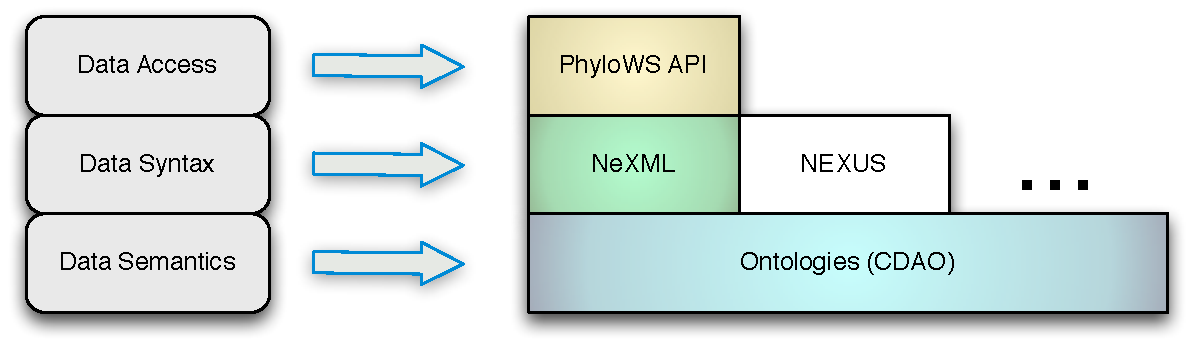
\includegraphics[width=0.6\textwidth]{EvoioStack.pdf}}
\caption{The EvoIO Stack}
\label{stack}
\end{figure}

\subsection*{Figure 2 - The Principle View of OTUs and Characters}
This figure summarizes the core concepts from phylogenetic analysis that
are captured by the CDAO ontology.

\begin{figure}[h]
\centerline{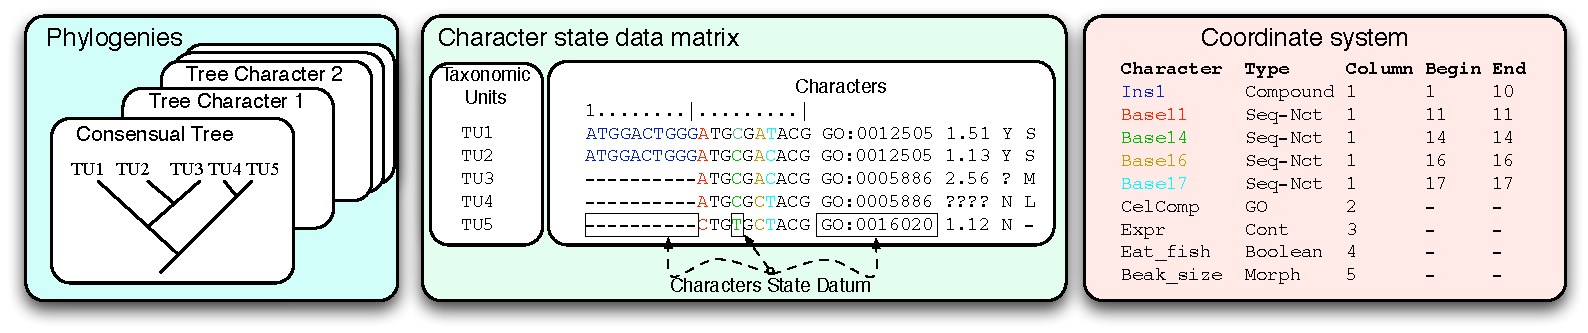
\includegraphics[width=0.9\textwidth]{cdofig.pdf}}
\caption{OTUs and Characters}
\label{cdao1}
\end{figure}

\subsection*{Figure 3 - Snapshot of the Key concepts of CDAO}
This figure provides a very small summary of the core concepts and relations
described in CDAO.

\begin{figure}[h]
\centerline{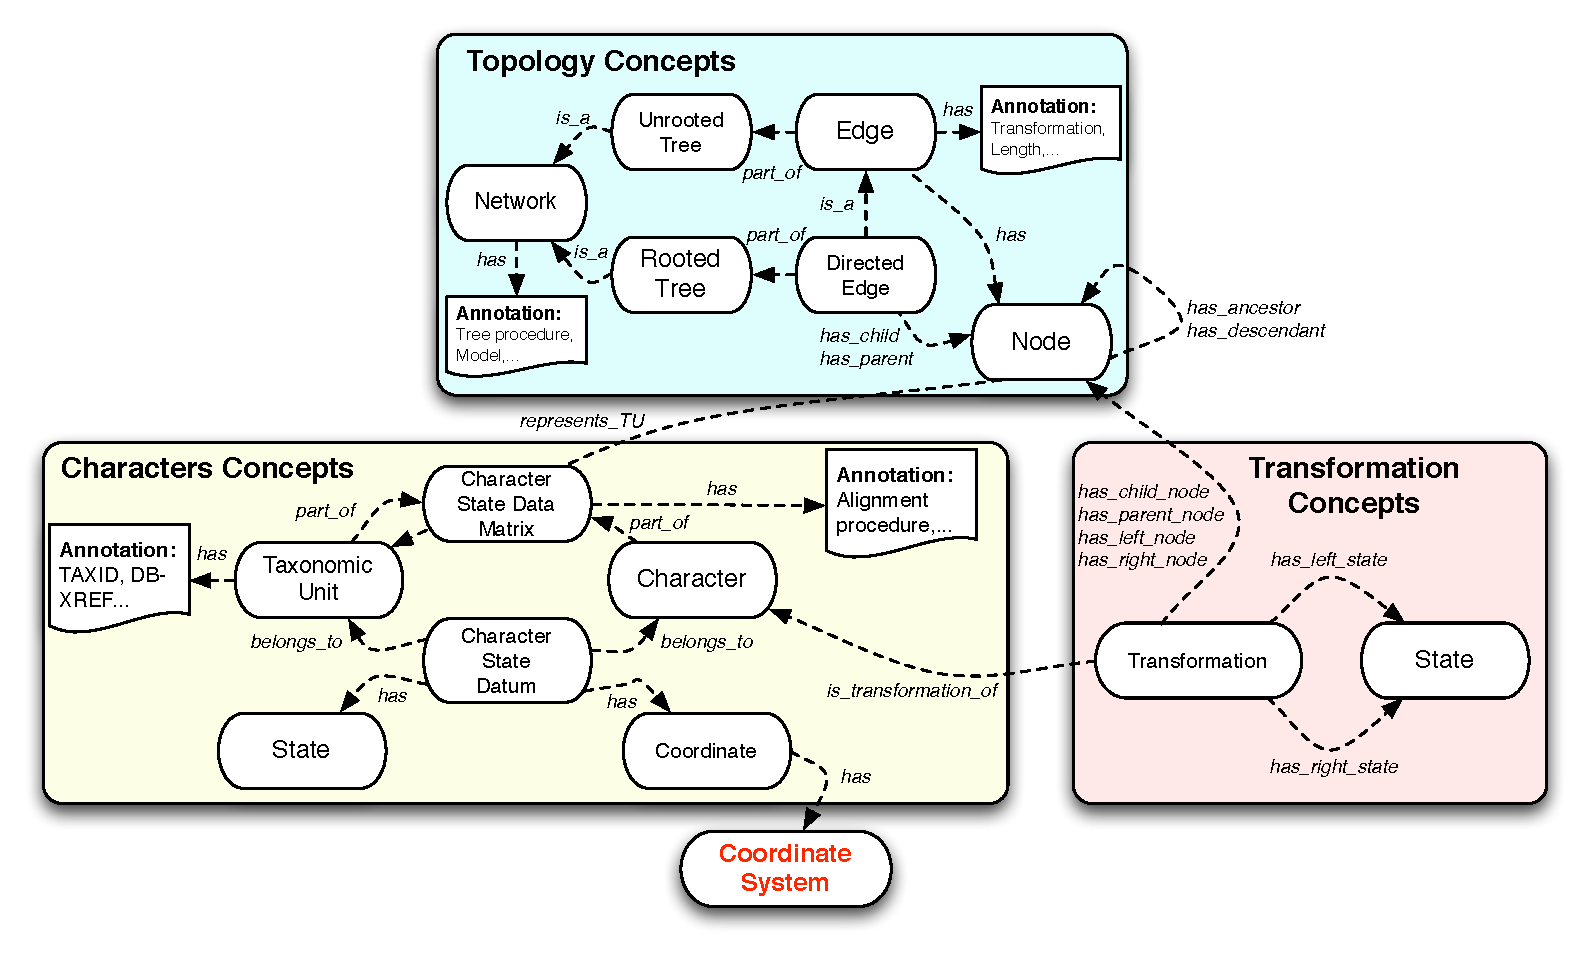
\includegraphics[width=0.8\textwidth]{cdao2.pdf}}
\caption{Core Concepts in CDAO}
\label{cdao2}
\end{figure}


  \subsection*{Figure 2 - TreeViewer with search}

      This is the TreeViewer Application displaying the tree Tree3099 from Treebase and searching for all nodes and edges with \#Ilex\_

%  \subsection*{Figure 2 - Sample figure title}
%      Figure legend text.



%%%%%%%%%%%%%%%%%%%%%%%%%%%%%%%%%%%
%%                               %%
%% Tables                        %%
%%                               %%
%%%%%%%%%%%%%%%%%%%%%%%%%%%%%%%%%%%

%% Use of \listoftables is discouraged.
%%
%\section*{Tables}
%  \subsection*{Table 1 - Sample table title}
%    Here is an example of a \emph{small} table in \LaTeX\ using  
%    \verb|\tabular{...}|. This is where the description of the table 
%    should go. \par \mbox{}
%    \par
%    \mbox{
%      \begin{tabular}{|c|c|c|}
%        \hline \multicolumn{3}{|c|}{My Table}\\ \hline
%        A1 & B2  & C3 \\ \hline
   %     A2 & ... & .. \\ \hline
  %      A3 & ..  & .  \\ \hline
 %     \end{tabular}
%      }
%  \subsection*{Table 2 - Sample table title}
%    Large tables are attached as separate files but should
%    still be described here.



%%%%%%%%%%%%%%%%%%%%%%%%%%%%%%%%%%%
%%                               %%
%% Additional Files              %%
%%                               %%
%%%%%%%%%%%%%%%%%%%%%%%%%%%%%%%%%%%

\section*{Additional Files}
  \subsection*{Additional file 1 --- TreeViewerSearch.jpg}
	This is Figure 1


\end{bmcformat}
\end{document}







